\section{Gorntak}\label{gorntak}

Tags: Personaggio Leggendario Alias: Il Gentile Creatore: Davide Luogo:
Valtara

\section{Gorntak}\label{gorntak-1}

\begin{center}\rule{0.5\linewidth}{0.5pt}\end{center}

\begin{figure}
\centering
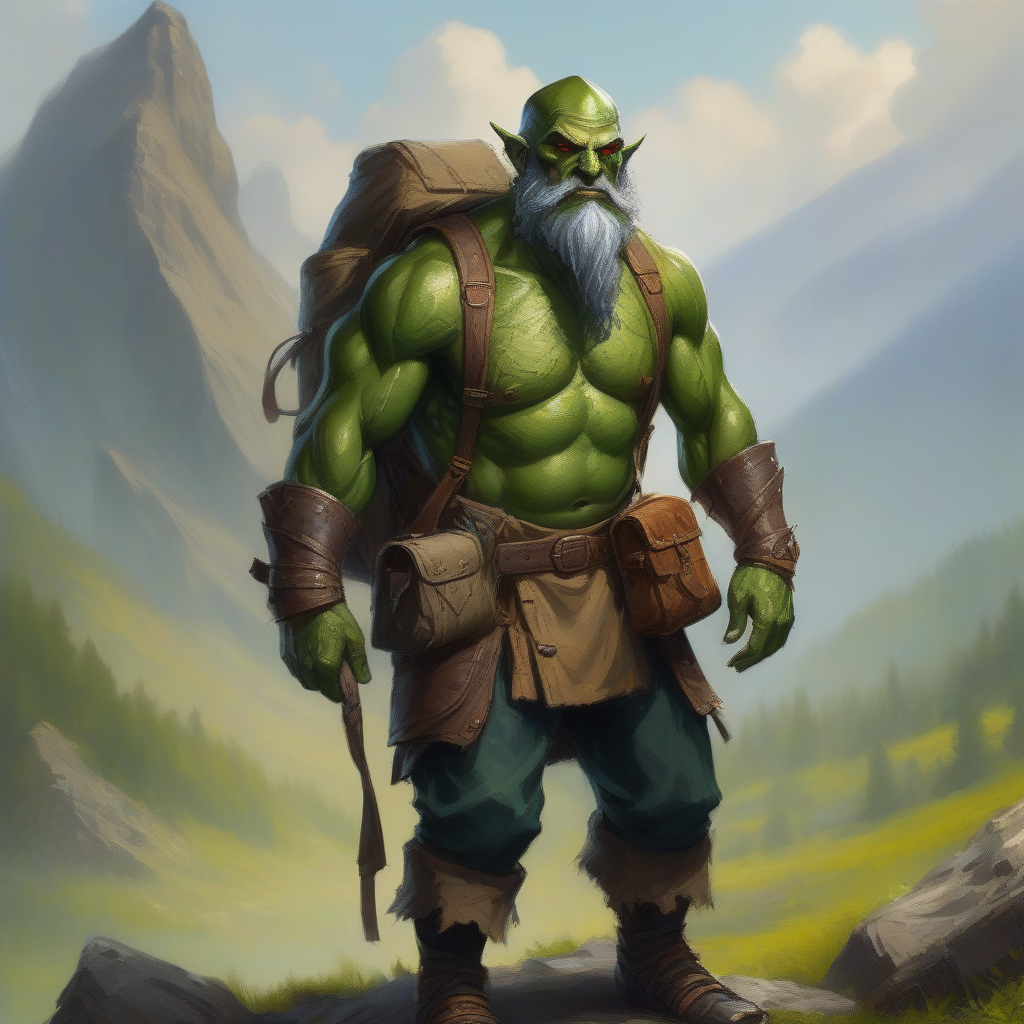
\includegraphics{create-an-image-of-gorntak-the-gentle-orc-picture-him-as-an-imposing-figure-tall-and-muscular-wi-3.png}
\caption{create-an-image-of-gorntak-the-gentle-orc-picture-him-as-an-imposing-figure-tall-and-muscular-wi-3.png}
\end{figure}

Informazioni Generali

Età: Sconosciuta

Data di nascita: Sconosciuta

Luogo di nascita: Valtara

Razza: Orco

\begin{center}\rule{0.5\linewidth}{0.5pt}\end{center}

\subsection{1. Descrizione Generale}\label{descrizione-generale}

\begin{center}\rule{0.5\linewidth}{0.5pt}\end{center}

\begin{figure}
\centering
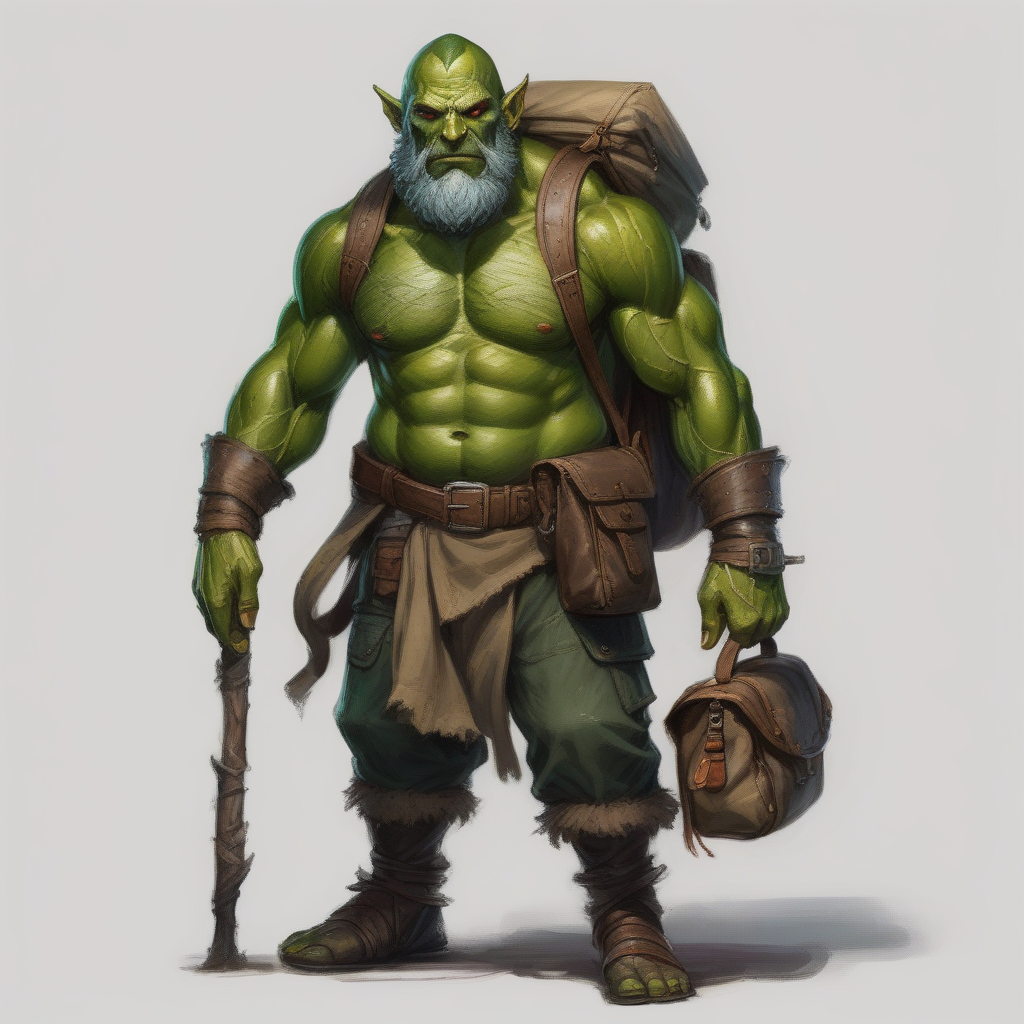
\includegraphics{create-an-image-of-gorntak-the-gentle-orc-picture-him-as-an-imposing-figure-tall-and-muscular-wi-4.png}
\caption{create-an-image-of-gorntak-the-gentle-orc-picture-him-as-an-imposing-figure-tall-and-muscular-wi-4.png}
\end{figure}

\emph{Gorntak}, noto come \emph{Il Gentile}, è stato un orco leggendario
nato in un villaggio tribale noto per la sua ferocia e brutalità.
Abbandonando la sua tribù in giovane età, Gorntak intraprese un
pellegrinaggio attraverso le terre di Valtara, diventando una figura
emblematica di altruismo e buone opere.

\begin{quote}
``Se ni mondo esistesse un po' di bene'' - Incipit della poesia
preferita di Gorntak
\end{quote}

\subsection{2. Biografia}\label{biografia}

\begin{center}\rule{0.5\linewidth}{0.5pt}\end{center}

\subsubsection{2.1 Infanzia e inizio del
pellegrinaggio}\label{infanzia-e-inizio-del-pellegrinaggio}

Gorntak trascorse la sua infanzia nel cuore di un villaggio orco noto
per la sua brutalità. Fin dalla giovane età, dimostrò di essere diverso
dai suoi coetanei. Mentre gli altri giovani orchi si immergevano
nell'addestramento bellico e nella competizione per dimostrare la loro
ferocia, Gorntak si ritirava spesso in solitudine, osservando con occhi
curiosi il mondo che lo circondava.

Ciò che lo distingueva era la sua innata curiosità e desiderio di
conoscenza. In segreto, si avventurava nei boschi circostanti, studiando
la flora e la fauna, cercando una connessione più profonda con la natura
che gli orchi spesso ignoravano. Questo atteggiamento non convenzionale
attirò sguardi sospettosi da parte degli altri membri della tribù, ma
Gorntak perseverò nella sua ricerca di un significato più elevato.

La svolta decisiva si verificò quando Gorntak assistette a un conflitto
violento tra la sua tribù e un gruppo di creature pacifiche che
abitavano le vicine colline. Mentre la tribù cercava di sopraffare
queste creature, Gorntak, spinto dal suo cuore gentile, intervenne
cercando di mediare una soluzione pacifica. Nonostante i suoi sforzi, la
situazione sfociò in uno scontro armato, lasciando Gorntak sconvolto per
la brutalità insensata.

Quell'evento segnò una rottura definitiva nella sua percezione del
mondo. Convinto che ci dovesse essere un modo diverso di vivere, Gorntak
prese la difficile decisione di abbandonare il suo villaggio natale. La
notte successiva, mentre gli altri dormivano, si avventurò
silenziosamente fuori dal villaggio, intraprendendo un pellegrinaggio
personale per scoprire un modo di vita che rispecchiasse i suoi ideali
di gentilezza e comprensione.

Così, iniziò il suo viaggio attraverso le terre di Valtara, determinato
a trovare un significato più profondo nella sua esistenza e a dimostrare
che gli orchi potevano essere più di meri predatori. Con ogni passo,
Gorntak si avvicinò sempre di più alla sua identità unica, sfidando le
aspettative della sua razza e lasciando dietro di sé un villaggio che,
pur ignorando il suo destino, non avrebbe mai dimenticato l'orco gentile
che avevano visto nascere.

\subsubsection{2.2 Vita da Pellegrino}\label{vita-da-pellegrino}

l pellegrinaggio di Gorntak attraverso le terre di Valtara fu un
percorso epico, intessuto di avventure e scoperte che avrebbero plasmato
la sua identità e la sua leggenda. Lontano dal suo villaggio natale,
Gorntak si immerse nelle regioni sconosciute di Valtara con un senso di
scoperta e un'apertura mentale che contrastava notevolmente con
l'approccio solitamente brutale degli orchi.

Durante il suo viaggio, Gorntak incontrò una vasta gamma di creature e
popoli, ognuno con le proprie tradizioni e storie. La sua gentilezza e
la sua volontà di aiutare i bisognosi lo resero una figura rispettata,
anche in luoghi dove la sua razza era spesso vista con sospetto. Si
guadagnò il soprannome di ``Il Gentile'' proprio per le sue azioni
compassionevoli e il suo impegno a proteggere coloro che non potevano
difendersi.

Il momento cruciale si verificò quando Gorntak si addentrò nella temuta
Foresta dei Giganti. Nonostante la sua fama di pericolosità, Gorntak,
con il suo coraggio e la sua astuzia, tracciò percorsi sicuri attraverso
il fitto degli alberi, rendendo accessibili le zone altrimenti
inesplorate della foresta. La sua abilità nel negoziare con le creature
selvagge e il suo rispetto per l'ambiente lo resero una figura
leggendaria tra gli abitanti delle terre selvagge.

\subsubsection{\texorpdfstring{2.3 \textbf{Scomparsa
Misteriosa}}{2.3 Scomparsa Misteriosa}}\label{scomparsa-misteriosa}

Dopo decenni di viaggi e gesti eroici, le tracce di Gorntak si persero
nel mistero. La sua scomparsa lasciò dietro di sé un vuoto nella
narrazione di Valtara, e le storie su di lui iniziarono a sbiadire col
passare del tempo. L'incertezza sulla sua sorte divenne parte integrante
del mito che circonda il suo nome.

\subsubsection{\texorpdfstring{2.4 \textbf{Eredità e Scomparsa dalla
Storia}}{2.4 Eredità e Scomparsa dalla Storia}}\label{eredituxe0-e-scomparsa-dalla-storia}

Sebbene Gorntak sia stato un'icona nel suo tempo, la sua figura è
gradualmente svanita dalla memoria collettiva nel corso dei secoli. La
sua eredità persiste solo in poche leggende tra tribù e villaggi, mentre
il suo nome è sempre più relegato all'oblio.

\subsection{3. Personalità}\label{personalituxe0}

\begin{center}\rule{0.5\linewidth}{0.5pt}\end{center}

La personalità di Gorntak era un'eccezione nel mondo degli orchi,
caratterizzata da una combinazione unica di forza e gentilezza.
Contrariamente alla brutalità tipica della sua razza, Gorntak era dotato
di un cuore generoso e compassionevole. La sua gentilezza emergeva
attraverso il suo impegno nel proteggere i deboli e nell'offrire aiuto a
coloro che ne avevano bisogno. Nonostante la sua forza imponente,
preferiva risolvere i conflitti attraverso la diplomazia piuttosto che
la violenza, guadagnandosi la fiducia e il rispetto di coloro che
incontrava. La sua natura altruista e il desiderio di creare un impatto
positivo nel mondo lo resero un personaggio straordinario,
distinguendolo nettamente tra le leggende degli orchi e lasciando
un'impronta indelebile nella storia di Valtara.

\subsection{A. Galleria Immagini}\label{a.-galleria-immagini}

\begin{figure}
\centering
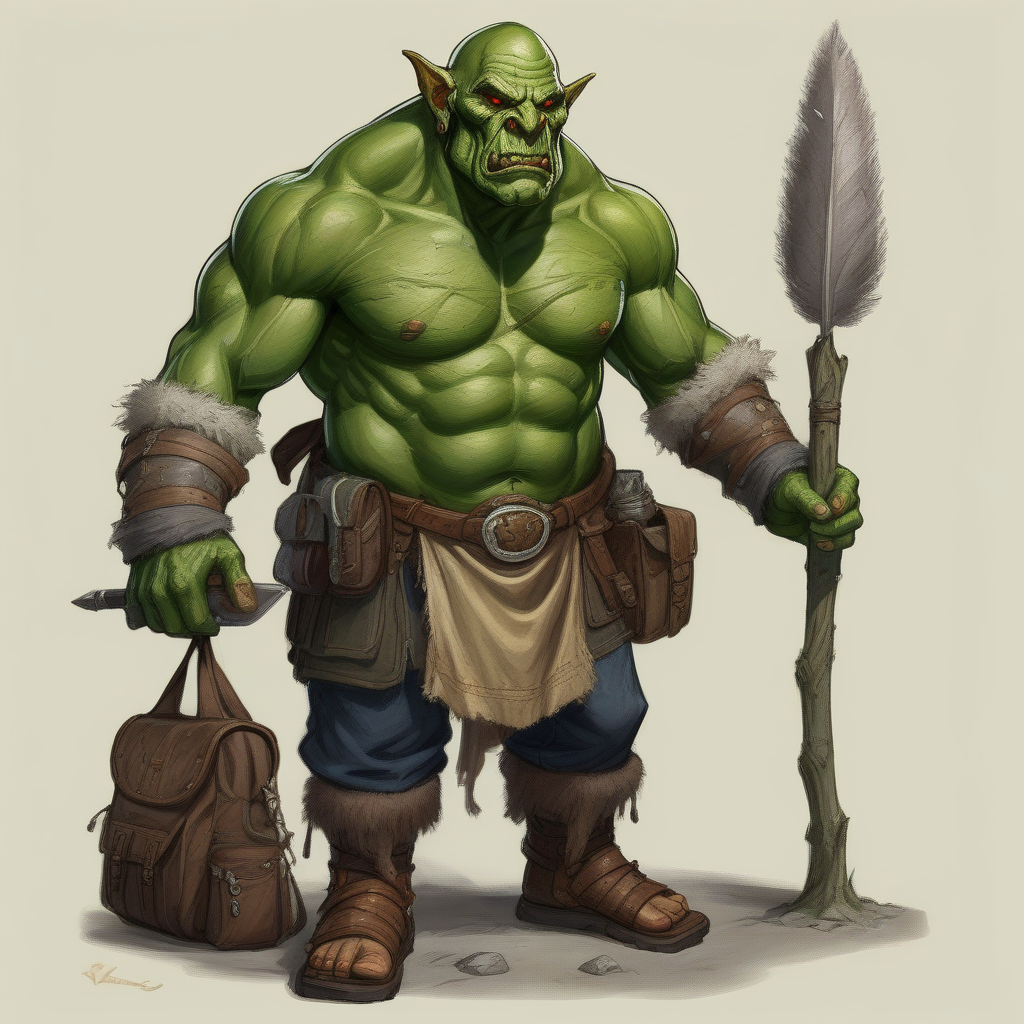
\includegraphics{create-an-image-of-gorntak-the-gentle-orc-picture-him-as-an-imposing-figure-tall-and-muscular-wi.png}
\caption{create-an-image-of-gorntak-the-gentle-orc-picture-him-as-an-imposing-figure-tall-and-muscular-wi.png}
\end{figure}

\begin{figure}
\centering
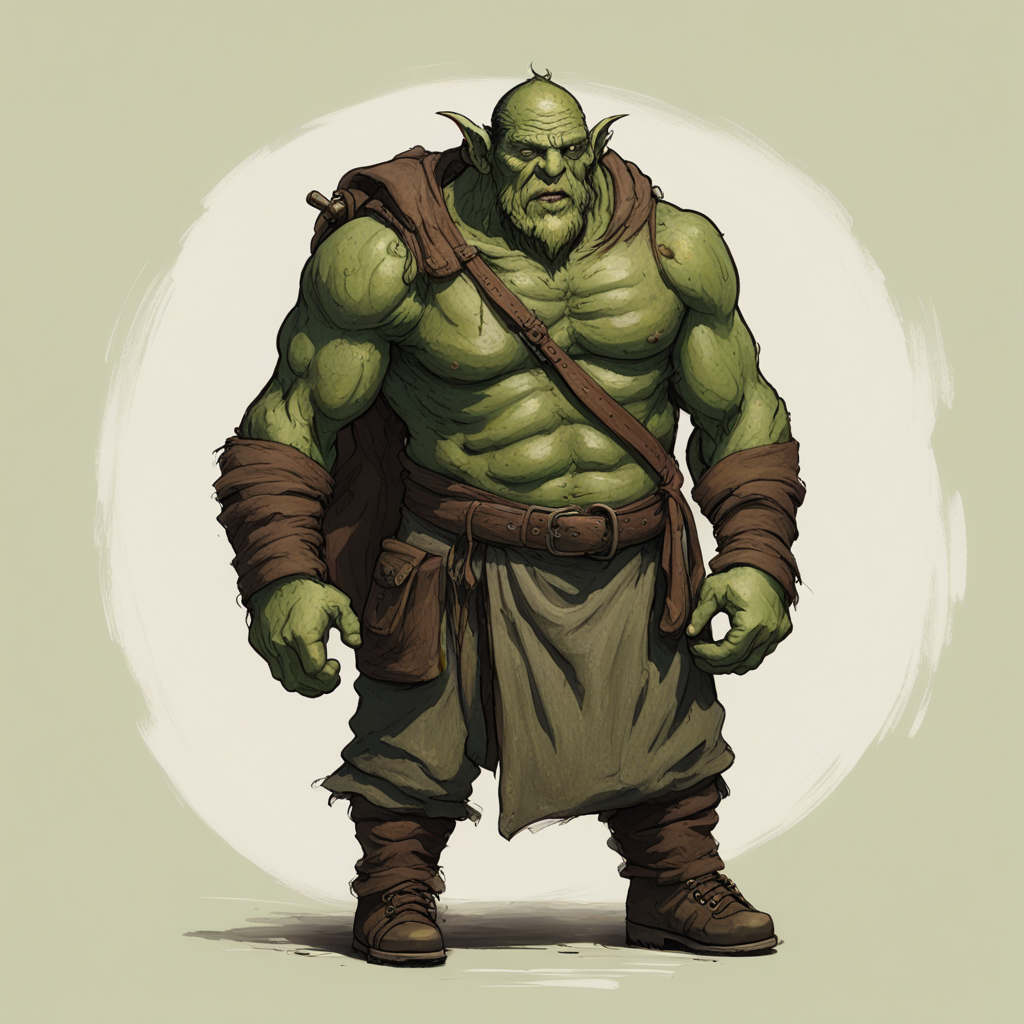
\includegraphics{create-an-image-of-gorntak-the-gentle-orc-picture-him-as-an-imposing-figure-tall-and-muscular-wi-2.png}
\caption{create-an-image-of-gorntak-the-gentle-orc-picture-him-as-an-imposing-figure-tall-and-muscular-wi-2.png}
\end{figure}

\begin{figure}
\centering
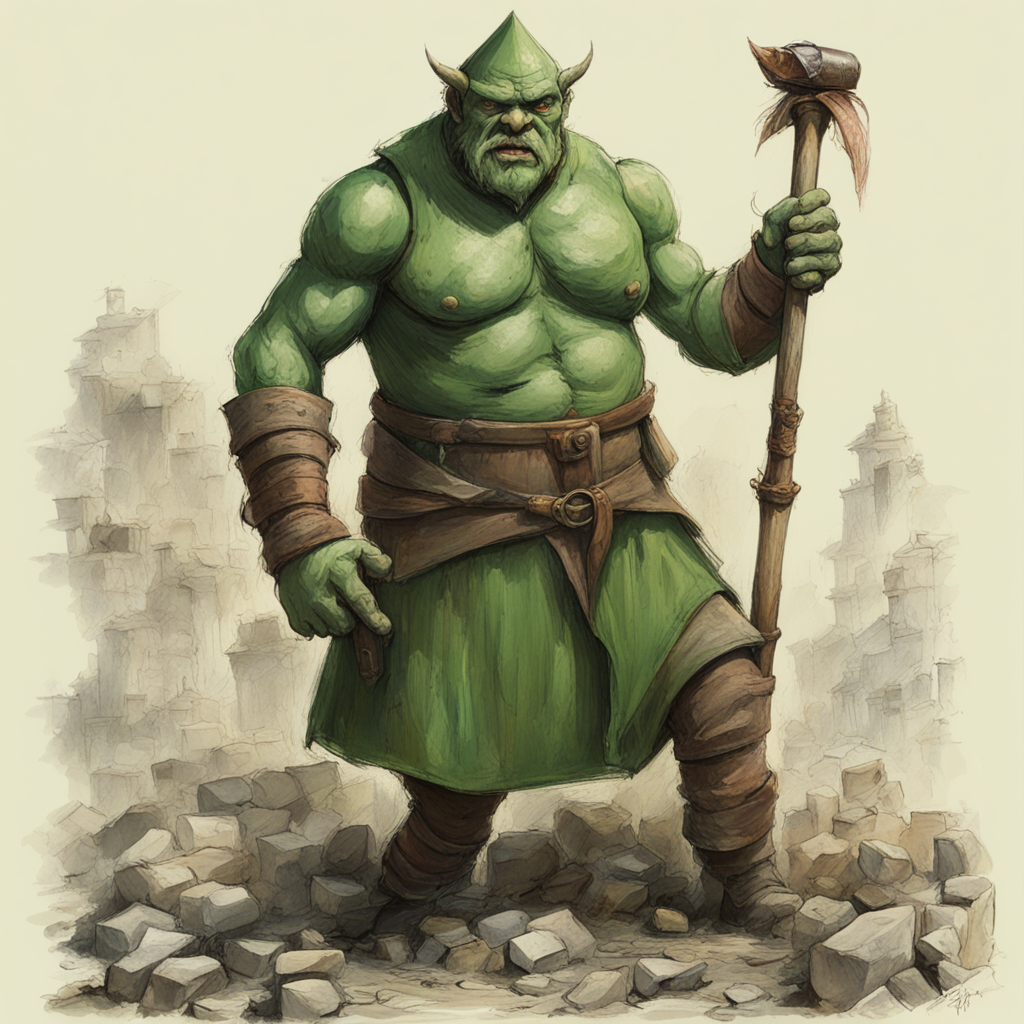
\includegraphics{crea-unimmagine-di-gorntak-lorco-gentile-immaginalo-come-una-figura-imponente-alta-e-muscolosa.png}
\caption{crea-unimmagine-di-gorntak-lorco-gentile-immaginalo-come-una-figura-imponente-alta-e-muscolosa.png}
\end{figure}
